\chapterimage{header.jpg}
\bigskip
\chapter{Building the SWAN}

\noindent SWAN uses the \textit{SWAN.EDT} file to read the grid (\textit{swan\_coord.grd}) and bathymetry (\textit{swan\_bathy.bot}) files. 
It is also possible to define a numerical grid within the \textit{SWAN.EDT} and indicate the bathymetry file that will be read and associated 
with the defined grid.
\bigskip

\noindent As an example, SWAN files will be created from the ROMS grid, but without the introduction of initial data,
as the implementation of a grid inside \textit{SWAN.EDT} is not trivial.
\bigskip

\noindent For SWAN boundary conditions, the wind fields will come from the WRF, as soon as
the waves generated are associated with the atmospheric systems represented in these simulations. Without the information
the boundary files information, the simulated waves will be generated only within the boundary of the domain, disregarding the energy that
is leaving or entering the grid.
\bigskip

\noindent We will use the MATLAB script, \textit{make\_swan.m}, to generate the files. The script is located at:
\bigskip

\begin{bashcode}
/home/name.surname/repositorio/SWAN_scripts
\end{bashcode}
\bigskip

\noindent As shown in Figure \textcolor{bleu_cite}{\ref{makeswan}}, the script has the following construction:
\bigskip

\begin{figure}[H]
    \centering
    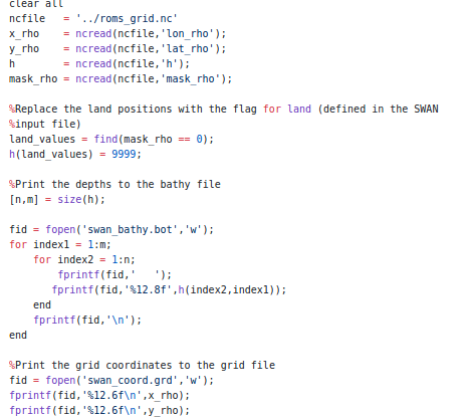
\includegraphics[width=0.47\textwidth]{makeswan.png}
    \caption{\textit{make\_swan.m} script.}
    \label{makeswan}
\end{figure}
\bigskip

\noindent To generate the two SWAN files, look in the script for the variable \textit{ncfile} and change the directory
to the path where your ROMS grid is.
\bigskip

\noindent Run the script and the two files will be created: \textit{swan\_coord.grd} and \textit{swan\_bathy.bot}.
The two files must be placed inside your project folder.
\bigskip

\chapter{Building the Budgell's Sea Ice Model}
\bigskip

\noindent The sea ice model is fully coupled to ROMS, so that, after generating the conditions of the
ROMS with ice data (see Section \textcolor{bleu_cite}{\ref{model2romssec}}), to activate the sea ice model 
just modify the ROMS \textit{.h} file in your project. According to \textcite{hedstrom2018}, you can
add the following options into the \textit{.h} file, as shown in Figure \textcolor{bleu_cite}{\ref{hiceroms}}:
\bigskip

\begin{itemize}
    \item \textbf{ICE\_MODEL}: defines the sea ice model;
    \item \textbf{ANA\_ICE}: defines initial analytical conditions for sea ice;
    \item \textbf{ICE\_THERMO}: defines the ice thermodynamics;
    \item \textbf{ICE\_MK}: defines the \textcite{Mellor1989} ice thermodynamics. Currently, is the only choice;
    \item \textbf{ICE\_MOMENTUM}: defines the momentum component of the ice;
    \item \textbf{ICE\_MOM\_BULK}: defines the alternate ice-water stress computation;
    \item \textbf{ICE\_EVP}: defines the elastic-viscous-plastic rheology from \textcite{Hunke1997} and \textcite{Hunke2001};
    \item \textbf{ICE\_QUAD\_STRENGTH}: defines the quadratic ice strength from \textcite{Overland1988};
    \item \textbf{ICE\_ADVECT}: defines the advection of ice tracers;
    \item \textbf{ICE\_SMOLAR}: defines the MPDATA use for ice tracers. Currently, it is the only option;
    \item \textbf{ICE\_UPWIND}: defines the upwind advection;
    \item \textbf{ICE\_BULK\_FLUXES}: define the ice part of bulk flux computation;
    \item \textbf{ICE\_DIAGS}: defines the diagnosis of sea ice;
    \item \textbf{ICE\_SHOREFAST} : defines the simple shorefast-ice algorithm from \textcite{Budgell2005};
    \item \textbf{ICE\_I\_O}: defines to allow light into the ice as heat;
    \item \textbf{ICE\_CONVSNOW}: defines the conversion of flooded snow to ice.
\end{itemize}
\bigskip

\begin{figure}[H]
    \centering
    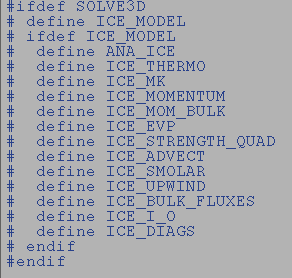
\includegraphics[width=0.3\textwidth]{hiceroms.png}
    \caption{Screenshot of ROMS \textit{.h} file}
    \label{hiceroms}
\end{figure}
\bigskip

\noindent For more information about the model, it is recommended to read \textcite{hedstrom2018}.
\bigskip

\noindent Get the \textit{.in} file for the sea ice model. Copy the file \textit{ice.in} into the Kerana repository and add it to your project.
\bigskip

\begin{bashcode}
    /home/name.surname/repositorio/ICE_scripts
\end{bashcode}
\bigskip
    
\noindent Modify the ROMS \textit{.in} file, pointing to the \textit{ice.in} into the variable \textit{IPARNAM}:
\bigskip

\begin{bashcode}
nedit ocean.in
IPARNAM =  ice.in
\end{bashcode}